\chapter{Dataset}\label{dataset}
\textit{by Florian Fallenbüchel}\\
The dataset which we will use in our experiments consists of 106574
songs, downloaded from the Free Music Archive~\cite{fma_dataset}. This
gives us 917 GB of Creative Commons-licensed audiofiles, tagged with the
respective genres. While a song may have multiple subgenres from a range
of 161 genres, the data set assigns a single top genre to each song. We
will use these top genres as labels in our experiments. There are 16
different top genres in the data, while some songs have tagged an empty
string.

\section{Distribution of the genres}

Figure~\ref{unfiltered} shows the genre distribution over the
full data set. Unfortunately, we realized too late, that the empty genre
is considered a class, and therefore, that the data is heavily
imbalanced. This influenced most of the experiments we did with the set,
delivering 53$\%$ accuracy for some of our neural networks, which only
predicted the empty genre. The individual chapters will provide more
insight.

\begin{figure}[!htb]
	\centering
	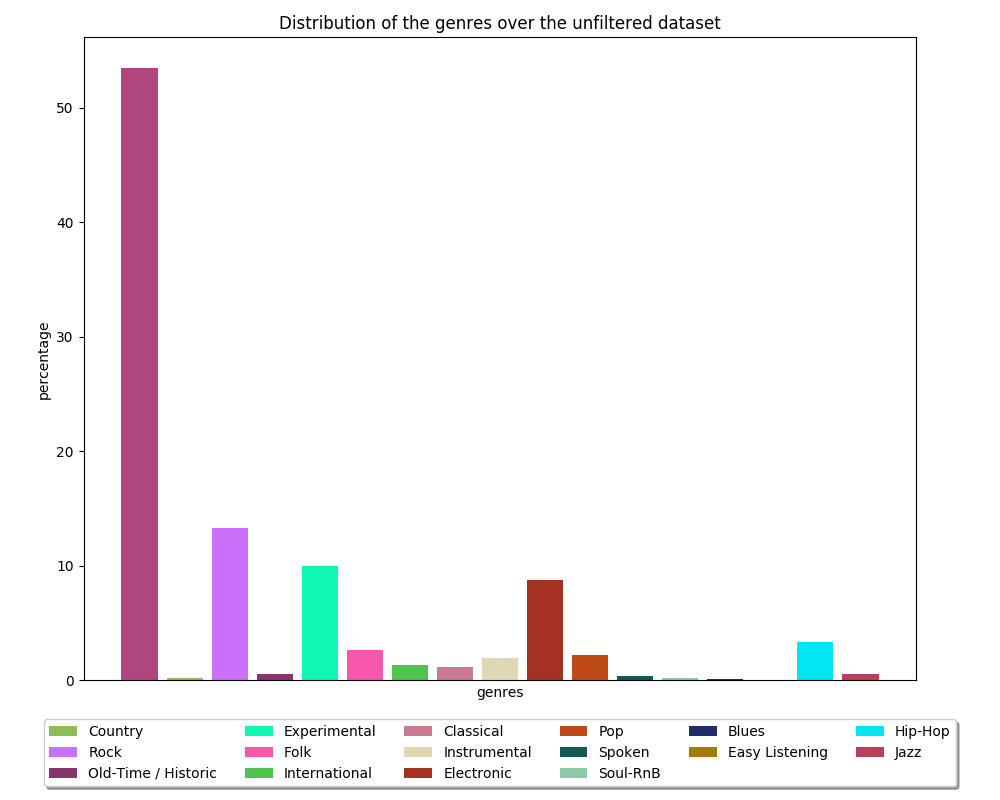
\includegraphics[width=1.0\textwidth]{images/genredist.png}
	\caption{Distribution of the genres over the dataset.
	About 53$\%$ of the data (left bar) has no top genre tagged.}
	\label{unfiltered}
\end{figure}

\begin{figure}[]
	\centering
	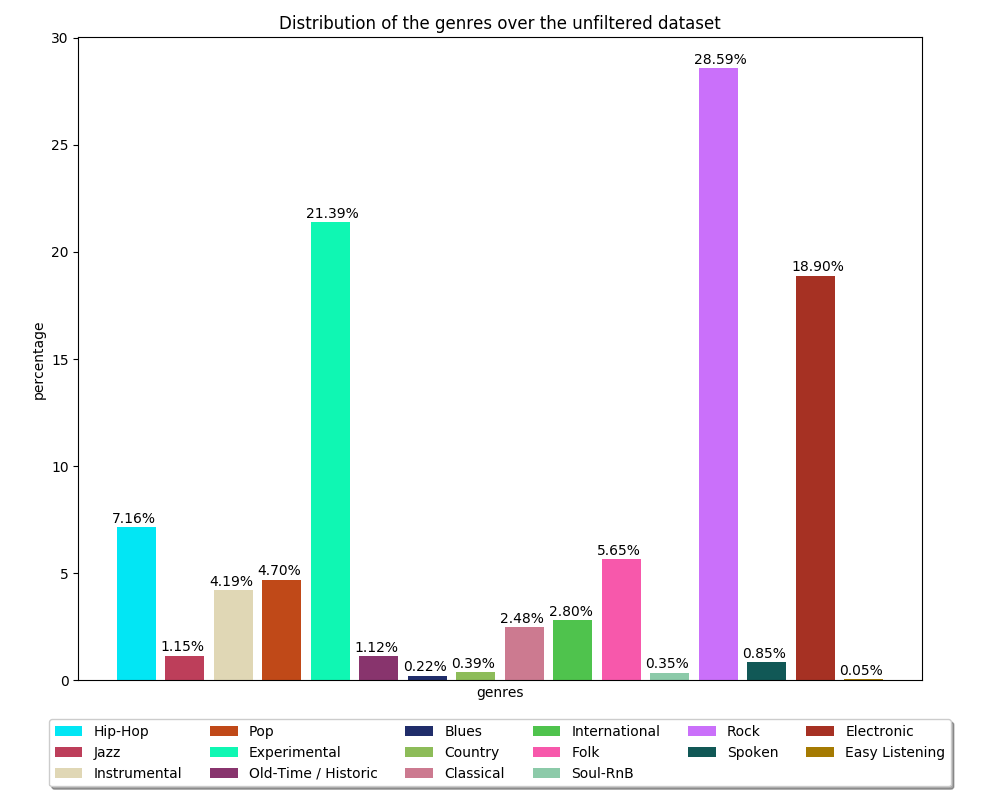
\includegraphics[width=1.0\textwidth]{images/genredistfiltered.png}
	\caption{Distribution of the genres over the filtered dataset with no empty
	top genre.}	
	\label{filtered}
\end{figure}

Therefore, we had to filter the songs from the set which were untagged,
as they hinder training not only by delivering high accuracy for the
prediction of a single class, but also, because the songs are probably
from one of the other 16 classes in reality and therefore have similar
features to the remaining songs, but a different tag. This leaves us
with 49598 songs from the original set. Figure~\ref{filtered} pictures
the distribution of the genres after the tracks with no top genre got
filtered out. As you can see, the data is still imbalanced, with a
majority of the songs being either Rock, Experimental or Electronic
music. To improve results in the future, we should filter out genres
with small sample sizes. Due to the deadline, we were only able to redo
some of our tests we already carried out on the full dataset.\\
We used 20\% of our data for testing, resulting in 39679 songs for
training and 9919 for validation (85260 and 21314 in the unfiltered data
set). As the dataset has an ordering of genres, due to tracks of the
same album usually being the same genre, we shuffle the data before
splitting to obtain a similar distribution over the two sets.
Figure~\ref{trainval} shows the genre distributions of our filtered
train and validation sets. As you can see, the genres are indeed equally
distributed for the two sets, but the classes themself are still
imbalanced. The distribution of the splits for the experiments carried
out with the unfilterd data set also follow the distribution of the
whole data in Figure~\ref{unfiltered}. This should be taking into
account while evaluating our accuracy statistics.

\begin{figure}
	\centering
	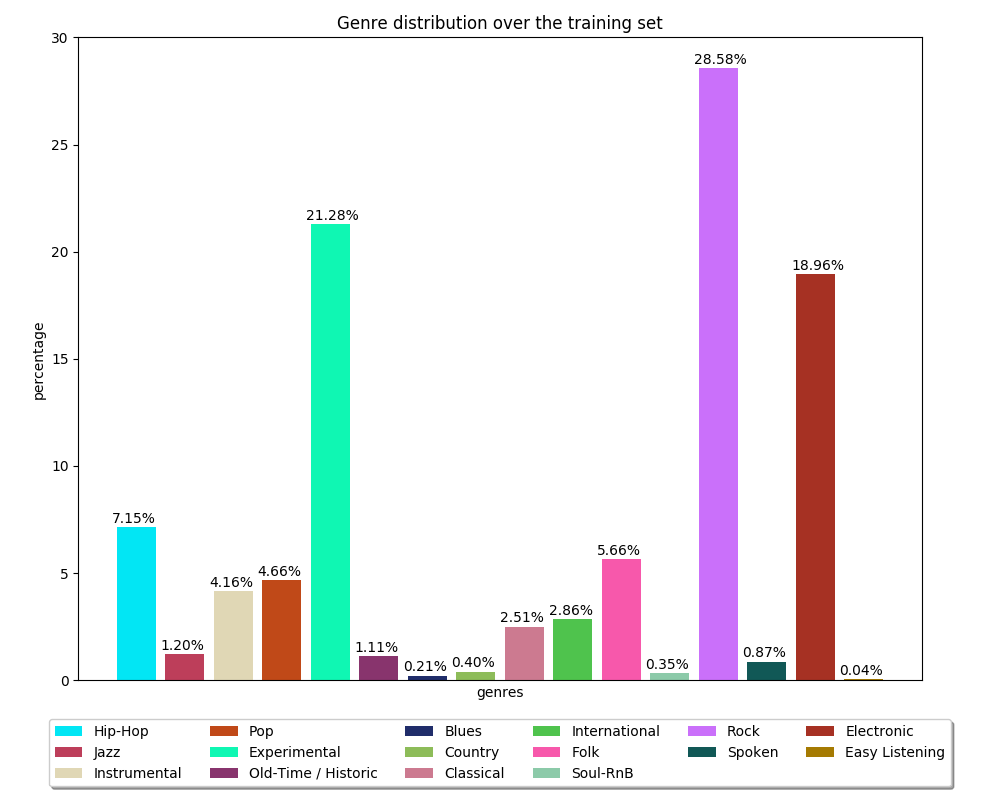
\includegraphics[width=1.0\textwidth]{images/train.png}
	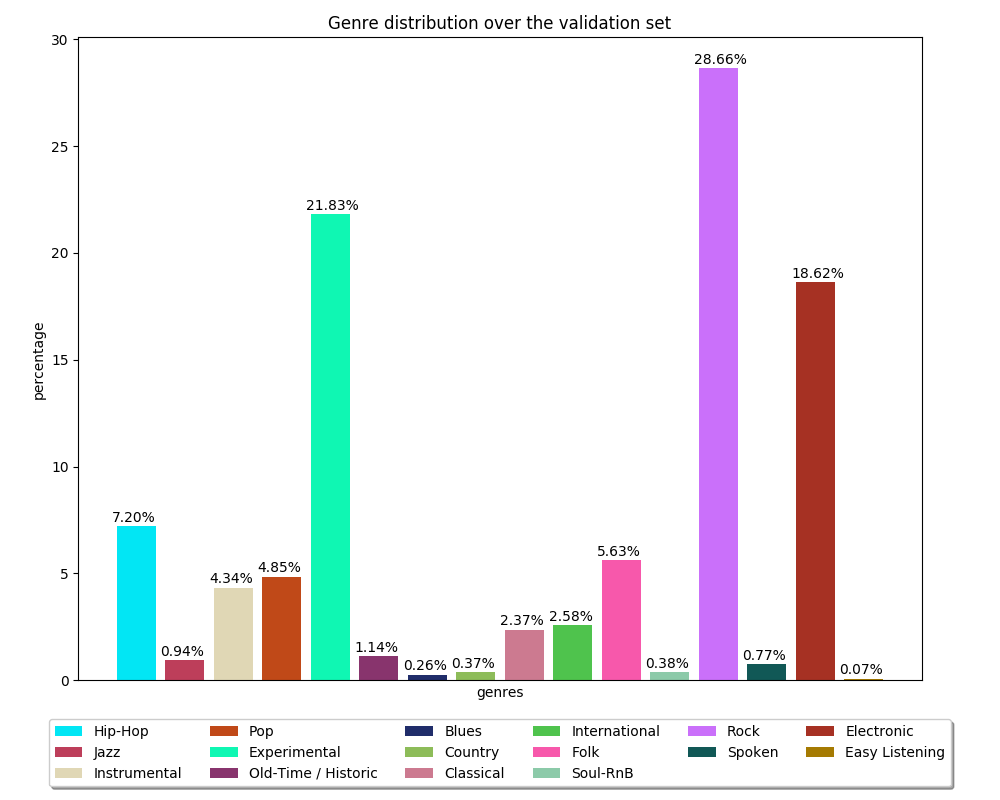
\includegraphics[width=1.0\textwidth]{images/val.png}
	\caption{Genre distribution over the training and validation
	sets. The two distributions are quite similar.}
	\label{trainval}
\end{figure}